\let\negmedspace\undefined
\let\negthickspace\undefined
\documentclass[journal]{IEEEtran}
\usepackage[a5paper, margin=10mm, onecolumn]{geometry}
%\usepackage{lmodern} % Ensure lmodern is loaded for pdflatex
\usepackage{tfrupee} % Include tfrupee package

\setlength{\headheight}{1cm} % Set the height of the header box
\setlength{\headsep}{0mm}     % Set the distance between the header box and the top of the text

\usepackage{gvv-book}
\usepackage{gvv}
\usepackage{cite}
\usepackage{amsmath,amssymb,amsfonts,amsthm}
\usepackage{algorithmic}
\usepackage{graphicx}
\usepackage{textcomp}
\usepackage{xcolor}
\usepackage{txfonts}
\usepackage{listings}
\usepackage{enumitem}
\usepackage{mathtools}
\usepackage{gensymb}
\usepackage{comment}
\usepackage[breaklinks=true]{hyperref}
\usepackage{tkz-euclide} 
\usepackage{listings}
% \usepackage{gvv}                                        
\def\inputGnumericTable{}                                 
\usepackage[latin1]{inputenc}                                
\usepackage{color}                                            
\usepackage{array}                                            
\usepackage{longtable}                                       
\usepackage{calc}                                             
\usepackage{multirow}                                         
\usepackage{hhline}                                           
\usepackage{ifthen}                                           
\usepackage{lscape}
\begin{document}

\bibliographystyle{IEEEtran}
\vspace{3cm}

\title{1 - 1.4 - 3}
\author{AI24BTECH11025 - PEDAPROLU LAKSHMI KUSHAL
}
% \maketitle
% \newpage
% \bigskip
{\let\newpage\relax\maketitle}

\renewcommand{\thefigure}{\theenumi}
\renewcommand{\thetable}{\theenumi}
\setlength{\intextsep}{10pt} % Space between text and floats


\numberwithin{equation}{enumi}
\numberwithin{figure}{enumi}
\renewcommand{\thetable}{\theenumi}


\textbf{Question:}

\textbf{Find the ratio in which the point \(P \) $\brak{\frac{3}{4}, \frac{5}{12} }$ divides the line segment joining the points \(A \) $\brak{\frac{1}{2},\frac{3}{2}}$ and \(B \) $\brak{2,-5}$.}
\\

\textbf{Solution:}\\
\begin{table}[h!]    
  \centering
  \begin{tabular}{|c|c|c|}
  \hline
        \textbf{Variable} & \textbf{Description}                                      & \textbf{Value}                          \\
        \hline
     
        $\vec{A}$      & Point $\vec{A}$ coordinates                                  & $\left(\frac{1}{2}, \frac{3}{2}\right)$ \\
        \hline
        $\vec{B}$      & Point $\vec{B}$ coordinates                                  & $\brak{2, -5}$                        \\
        \hline
        $\vec{P}$ & Point $\vec{P}$ coordinates & $\left(\frac{3}{4}, \frac{5}{12}\right)$ \\
        \hline
        $\vec{m}$ & Ratio part for point $\vec{B}$  & $5$  \\
        \hline
        $\vec{n}$      & Ratio part for point $\vec{A}$  & $1$  \\
        \hline
        \textbf{Ratio}    & Ratio in which point $\vec{P}$ divides line segment $\vec{AB}$  & $5:1$                          \\
        \hline
        
    \end{tabular}
  \caption{Variables Used}
  \label{tab}
\end{table}
To find the ratio \( m : n \) in which the point \( P\left(\frac{3}{4}, \frac{5}{12}\right) \) divides the line segment joining the points \( A\left(\frac{1}{2}, \frac{3}{2}\right) \) and \( B(2, -5) \), we use the section formula.

Let the ratio be \( m : n \).
\begin{align}
\left( \frac{m \cdot x_2 + n \cdot x_1}{m+n}, \frac{m \cdot y_2 + n \cdot y_1}{m+n} \right) \\
\left( \frac{m \cdot 2 + n \cdot \frac{1}{2}}{m+n}, \frac{m \cdot (-5) + n \cdot \frac{3}{2}}{m+n} \right) = \left(\frac{3}{4}, \frac{5}{12}\right) \\
\frac{m \cdot 2 + n \cdot \frac{1}{2}}{m+n} = \frac{3}{4} \\
\frac{m \cdot (-5) + n \cdot \frac{3}{2}}{m+n} = \frac{5}{12} 
\end{align}

$ m\cdot8 + n\cdot2 = m\cdot3 + n\cdot3 $\\
Hence , the answer is \textbf{1:5} .

\begin{figure}[h]
	\centering
	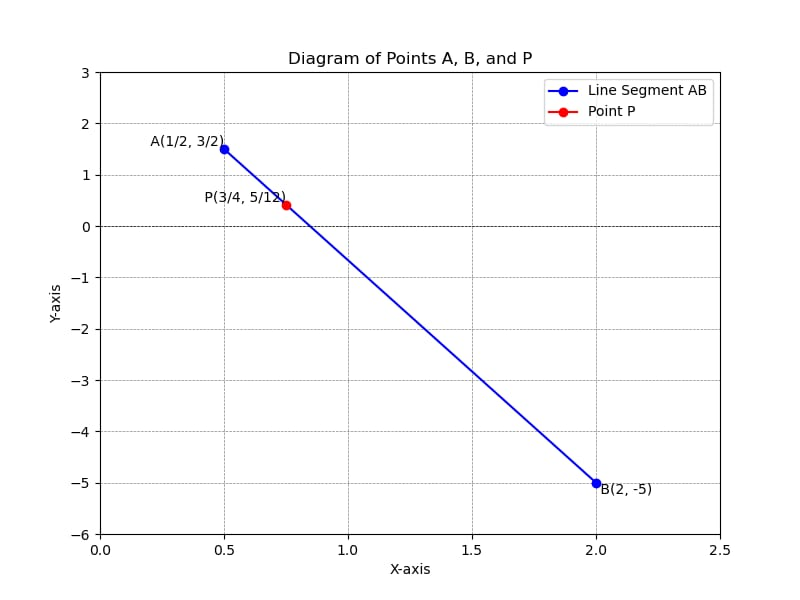
\includegraphics[scale=0.4]{IMG.jpg}
	\label{Fig}
\end{figure}

\end{document}